% TARI29_Assignment_report_template.tex
% This is a template for the assignment reports
% TARI29 Artificial Intelligence, 7.5 credits, Winter 2024
% Original version by:  Vladimir Tarasov, 2024
% Revised by:           Alexandros Tzanetos, 2024 

% Use a modern class instead of an old article class
\documentclass{scrartcl}

\KOMAoptions{
    parskip=half,  % full, off
    fontsize=12pt, % base font size (10pt default)
    % headings=big,% small/normal/big headings (normal is default), 
    % paper=a5,    % paper format (a4 default) 
    pagesize=auto  % Use paper format for PDF too
}

% ---------------------- Report details --------------------- %
%\newcommand{\docauthor}{Name1, Name2, Name3, Name4}
\newcommand{\courseyear}{2024}
\newcommand{\coursename}{TARI29 Artificial Intelligence}
\newcommand{\coursecredits}{7.5 credits}
\newcommand{\fullcoursename}{\coursename, \coursecredits}
\newcommand{\termname}{Winter \courseyear}
\newcommand{\groupnumber}{\#}
\newcommand{\reportname}{Group 7 Assignment Report}
\newcommand{\assignmentname}{Evolutionary Computation Assignment}
% ------------------ End of report details ------------------ %



% ---------- Setting up properties of the PDF file ---------- %
\usepackage{hyperref}
\hypersetup{
    colorlinks=true,
    allcolors=blue,
    pdftitle={\reportname},
    pdfauthor={Name1, Name2, Name3, Name4},
    pdfsubject={\coursename, \termname}
	% pdfpagemode=FullScreen,
	% pdfpagemode= UseOutlines % the default if present
}
\usepackage{hyphenat}
% ------------ End of properties of the PDF file ------------ %



% ----------- Setting up the headers and footers ------------ %
\usepackage{scrlayer-scrpage}
\pagestyle{scrheadings}
\KOMAoptions{% 
    headsepline,% line below the header
    plainheadsepline,% also on scrplain
}
\clearscrheadfoot % Erase all current configurations
% inner part of the header [titel_page]{other_pages}
\ihead[\coursename, \courseyear]{\coursename, \courseyear}
% outer part of the header [titel_page]{other_pages}
\ohead{\assignmentname}
% center part of the footer [titel_page]{other_pages}
\cfoot[\textup{Page \pagemark\ of \ztotpages}]{\textup{Page \pagemark\ of \ztotpages}}
% ------------- End of the headers and footers -------------- %



% ---------------- Setting up the title page ---------------- %
\title{\reportname}
\subtitle{An Evolutionary Algorithm for the N-Queen problem}
%\author{\docauthor}
\author{Sandra Carlsson\quad Besan Ewir \\ Eddie Olofsgård\quad Ebba Brage}
\date{\today}
% ------------------ End of the title page ------------------ %



% --------------- Packages and custom commands -------------- %
% Specify the input encoding of the source file as UTF8 
\usepackage[utf8]{inputenc}
% The T1 font encoding is an 8-bit encoding and fully supports words containing accented characters
\usepackage[T1]{fontenc}
% Load Latin modern fonts in outline format
\usepackage{lmodern}
% Load better typewriter font
\usepackage{inconsolata}
% For better hyphenation patterns
\usepackage[english]{babel}
% For improved micro-typography
\usepackage{microtype}
% Switch off extra space after a sentence
\frenchspacing
% To be able to iclude pictures
\usepackage{graphicx}
\usepackage{zref-totpages} % To get the total number of pages
\usepackage{mathtools,amsmath} % for advanced math formulas
 % To highlight source code
\usepackage{minted}
% Default options for all minted environments
\setminted{
           style=default, % for minted envronment
           autogobble, % automatically remove all common leading whitespace
           xleftmargin=10pt, % indentation to add (on the left) before the listing
           numbersep=6pt, % gap between numbers and start of line
           linenos, % enables line numbers
           mathescape % enables the usual math mode inside comments
}
\setmintedinline[c]{style=default} % for minted inlines
% Flexible handling of verbatim text
\usepackage{fancyvrb}
% For well-spaced lines and guidelines in tables
\usepackage{booktabs}
% To typeset algorithms or pseudocode in LaTeX 
\usepackage{algorithm}
\usepackage{algpseudocode}
% For plots and graphs
\usepackage{pgfplots}
\pgfplotsset{width=10cm,compat=1.9}

% To generate placeholder text - can be deleted when you have written real text
\usepackage{lipsum}
% ----------- End of packages and custom commands ----------- %


\begin{document}

\maketitle

% % It can be commented out if you do not want the table of contents
% \tableofcontents 


\section{Introduction}
\label{sec:intro}

\textcolor{black}{This report presents the N-Queens problem and a generic algorithm that solves the problem. The problem is a common optimization problem where the goal is to place $n$ queens on a $n \times n$ chessboard and make sure there are no conflicts where the queens can attack each other vertically, horizontally or diagonally. The history of the problem is famous for its complexity when the value on $n$ increases. The solution that has been implemented includes initialization, selection, recombination and mutation which will be described in the following sections. The report further presents experimental results comparing the algorithm’s performance on different board sizes.}


\section{Problem}
\label{sec:problem_description}
\textcolor{black}{\textbf{What is the N-Queens Problem?\\} In the chess game of queens, we wish to place $n$ queens on an $n \times n$ chessboard in such a way that no queen can attack another, either horizontally, vertically, or diagonally. It originated from 8-Queens puzzle (introduced by Max Bezzel in 1848), and was later generalized to N-Queens problem. This was considered by several mathematicians in the 19th century, including Gauss and Nauck. In 1850, Nauck was the first to identify all 92 valid solutions to the 8-Queens problem. These 92 solutions can be reduced to 12 unique solutions when rotations and reflections are considered equivalent. \\ \\ The N-Queens problem is not only a mathematical challenge. It is furthermore an NP-hard problem with a solution space that grows exponentially with the number of queens. For small numbers of queens, brute force or backtracking can be used as exact methods but for larger n, they become too slow rapidly. As a result, the N-Queens problem is considered one of the main benchmarks for algorithm development and the artificial intelligence field.Besides optimization, the problem is also used in the scheduling field, circuit design, graph theory, air traffic control, and data compression.}

\textcolor{black}{\textbf{Motivation – Why Evolutionary Algorithms/ Motivation behind the evolutionary approach?\\} Because of its complexity, the N-Queens problem is typically approached with heuristic rather than exact methods. The use of evolutionary algorithms, specifically genetic algorithms (GA) is well suited to such a problem. They are able to efficiently traverse vast solution spaces, adapt to complex fitness landscapes, and bypass local optima through mechanisms such as crossover and mutation. \\ \\ According to previous research, genetic algorithms have been verified to be efficient for N-Queens problem. For example, Sarkar \& Nag \cite{sarkar2018nqueens} used a traditional GA along with a fitness function specially designed for the problem and achieved good outcomes even for larger values of n. In another study, Cao et al \cite{cao2020parallel} developed a parallel GA that was combined with simulated annealing, which enabled solving very large instances on GPU clusters. Similarly, Sharma \& Jain \cite{sharma2021novelMutation} came up with a better mutation strategy that repositions queens with the most conflicts, thereby drastically reducing the running time. \\ \\ These studies demonstrate that evolutionary algorithms are effective solution for N-Queens problem, but the results also reveal that performance depends largely on the design features of the algorithm. Based on this, our approach introduces a heuristic-based initialization that reduces diagonal conflicts early, providing a stronger foundation for optimization process. The population initialization is a greedy heuristic algorithm that places queens at the best available square in each row. This enables stronger starting boards than random shuffling. The swap mutation was chosen since it preserves the properties of unique columns and rows of the permutation representation. For parent selection, we used tournament selection (k=3) to balance selective pressure and diversification and avoid early convergence compared to elitist rank-based choice. Lastly, we applied single-point crossover with repair to maintain valid permutations (one queen per column) and maintain efficient search within the solution space. }

\textcolor{black}{\textbf{Mathematical Formulation \\} The N-Queens problem can be presented as a permutation problem. Any valid configuration is a permutation of the set $[0,1,2,\dots,n-1]$, where the value of each element $ci$ denotes the column position of the queen in row $i$. By doing this, it is guaranteed that no two queens occupy the same row or column. \\ \\ The remaining challenge is to avoid diagonal conflicts. This can be expressed mathematically as: \\ \[ |c i - c j| \neq |i - j| \text{ for all } |i \neq j| \] where $ci$ and $cj$ are the column positions of the queens in rows $i$ and $j$. If the condition is broken, it is such a case that two queens are lying on the same diagonal and can attack each other. \\ \\ This problem is classified as NP-hard, which implies that the number of potential permutations increases as $n!$. Consequently, brute force becomes impractical for larger instances. To solve this problem, heuristic methods are used to limit the search space. \\ \\ In our implementation, a heuristic initializer is applied to generate starting solutions. At each step, the algorithm selects a column with the least threat level, which minimizes the risk of diagonal conflicts. This provides a stronger preliminary point for the genetic algorithm to be further optimized. }

\section{Algorithm}
\label{sec:algorithm}

\textcolor{black}{\textbf{Initialization \\} To create the initial boards for the main loop a heuristic greedy algorithm is used. The algorithm goes through each row and places the queen randomly among the squares with the smallest number of queens that can attack it. If a column index has already been used, then it removes it randomizes again for the same row. If all squares of the smallest conflict value are occupied, then it moves on to the next to smallest conflict value. It then cycles through all rows creating a board with unique column indexes. Since the number of conflicts have been minimized compared to a completely random permutation the board leading to fewer generations needed to reach a final solution.}

\textcolor{black}{\textbf{Selection \\} In the initial setup of the algorithm, a straightforward rank-based elitist selection method was applied. The population got sorted by fitness levels, and the top 50 percent of individuals were kept on as parents. This approach made sure that the strongest performers consistently survived. Still, it came at a cost, cutting down on genetic variety and raising the chances of getting stuck too early in a suboptimal solution. \\ \\ To fix that issue, the refined version switched over to a tournament selection process. For every tournament, a small random group of candidates was pulled from the overall population. Then, the one with the lowest fitness score, meaning the least number of conflicts, was selected as a parent. The tournament size stayed steady at three. That choice strikes a reasonable balance. Bigger tournaments ramp up the pressure to pick the best, but they can limit diversity. Smaller ones keep things more varied, though selection gets looser. In our configuration, we select a number of parents equal to the population size ($parents\_count = gen\_size$), whereas the function’s default (if unspecified) keeps half of the population (at least two). This setup guarantees enough options for the next steps in recombination and mutation. \\ \\ The final design skipped elitism on purpose. Sure, elitism accelerates convergence by directly carrying over the top individuals without changes. But it also reduces the randomness, which might trap the process in early convergence. Instead, selective pressure was managed through the tournament size, while genetic diversity was sustained by mutation. As a result, even the fittest individuals had a high probability of being selected, but their survival was not guaranteed. This promotes more exploration and helps avoid getting premature stagnation.}

\textcolor{black}{\textbf{Recombine \\} This section of the algorithm is responsible for manipulating the board by combining two boards. It starts by looping through the boards. The first half of the current board (board A) is combined with the second half of the next board in the list (board B). The last board in the list will wrap around and combine with the first one. \\ \\ When two boards are combined, it’s possible for duplicate numbers to occur which makes the board invalid. To avoid this, the new board will run through a repair function. This function looks for missing and repeating numbers in the list representing the board. Repeating numbers in the second half of the board are replaced by the missing numbers, ensuring that each number appears exactly once and that the board is valid. \\ \\ Before moving on to the next board, a second board will be created in the same way but using the remaining halves of the initial boards (first half of board B and second half of board A). This will bubble the number of boards compared to before but since the count was halved in selection this will restore it.}

\textcolor{black}{\textbf{Mutation \\} The mutation function was implemented by two functions, \texttt{mutate} and \texttt{mutate\_extended}. The overall purpose of this algorithm is to prevent the population from becoming too homogeneous by continuously introducing new solutions. By maintaining variation, mutation also prevents the algorithm of getting trapped in local optima. \\ \\ The \texttt{mutate} function was implemented to swap places of two random positions in a board and was run by a given mutation rate where every board had a chance to be mutated. If there were a mutation, two indexes in the board swapped places and this approach are an effective way to maintain diversity in the population. \\ \\\texttt{mutate\_extended} is a developed version of the mutate function where the purpose is to create copies of the mutated individuals and gather them in a separate list. This leads to the preservation of the original population, while new mutated individuals are created to complement it. In this way, promising solutions are not lost during mutation. \\ \\The mutation rate is crucial for both functions in different ways. In the \texttt{mutate} function a high mutation rate may remove promising solutions because the function is random and not managed by fitness function. The \texttt{mutate\_extended} function does not remove promising solutions but it can become inefficient if too many random solutions are introduced. In this algorithm the mutation rate was set relatively low to keep a balance in the overall population and uses both functions to keep that balance. The purpose of using this mechanism is to keep generic variation and strive for a better solution by continuously implementing new variations to the population.}

\textcolor{black}{\textbf{Board representation \\} TBA}

\begin{algorithm}[H]
\caption{Genetic Algorithm for the N-Queens Problem}\label{alg:nqueens}
\begin{algorithmic}
\Require $n$, $gen\_size$, $mutation\_rate$, $max\_generations$, $stall\_limit$, $population\_init\_algorithm$
\Ensure A board with fitness $=0$, or the best configuration found if stagnation occurs
\State $generation\_num \gets 0$
\State $stall \gets 0$

\If{$population\_init\_algorithm = 0$}
    \State $generation \gets$ $gen\_size$ random boards
\ElsIf{$population\_init\_algorithm = 1$}
    \State $generation \gets$ $gen\_size$ heuristic boards
\Else
    \State \Return Error
\EndIf

\State $scored \gets$ list of $(candidate, fitness(candidate))$ for each candidate in $generation$

\ForAll{$(board, fit) \in scored$}
    \If{$fit = 0$}
        \State \Return $(board, 0, 0)$ \Comment{Perfect solution in the initial generation}
    \EndIf
\EndFor

\State $(best\_board, best\_fitness) \gets$ best element in $scored$

\While{$generation\_num < max\_generations$}
    \State $generation \gets$ \Call{tournament\_select}{$scored, 3, gen\_size$}
    \State $generation \gets generation \cup$ \Call{recombine}{$generation$}
    \State $generation \gets generation \cup$ \Call{mutate\_extend}{$generation, mutation\_rate$}
    \State $scored \gets$ list of $(candidate, fitness(candidate))$ for each candidate in $generation$
    \State $(cur\_best\_board, cur\_best\_fitness) \gets$ best element in $scored$

    \If{$cur\_best\_fitness = 0$}
        \State \Return $(cur\_best\_board, generation\_num, stall)$
    \EndIf

    \If{$cur\_best\_fitness < best\_fitness$}
        \State $best\_board \gets cur\_best\_board$
        \State $best\_fitness \gets cur\_best\_fitness$
        \State $stall \gets 0$
    \Else
        \State $stall \gets stall + 1$
        \If{$stall \geq stall\_limit$}
            \State \Return $(best\_board, generation\_num, stall)$
        \EndIf
    \EndIf

    \State $generation\_num \gets generation\_num + 1$
\EndWhile

\State \Return $(best\_board, generation\_num, stall)$
\end{algorithmic}
\end{algorithm}

\section{Experimental part}
\label{sec:experimentation}

\textcolor{black}{The algorithms and the hardware used for the experiment. The experiments were performed on a AMD Ryzen 7 5700X 8-Core Processor. With a clock frequency of 3401 Mhz. The algorithm that was outlined in the algorithm section is implemented in python at \href{https://github.com/Sneakycloud/N-queens\_problem\_Evolutionary\_Alg/tree/main}{github}. The repository also includes a "Base algorithm" folder where a simple evolutionary algorithm is included.}

\textcolor{black}{The simple algorithm is designed in a less sophisticated manner.}
\begin{itemize}
	\item Representation: It uses the same ordered list representation as the main algorithm. However, it does not guarantee that all column indexes are unique throughout the algorithm.
	\item Population initialization:  Creates a list with values 0 to n-1 and then shuffles the order.
	\item Recombination: Selects a start and end index within the length of the first parent. The selected interval of the first parent is combined the missing indexes from the second parent to create a child.
	\item Mutation: Randomly adds or subtracts one from a random index as long as the result is within bounds.
	\item Selection: Randomly picks boards from the old generation until the new generation is filled to the specified limit.
	\item fitness: In addition to calculating the diagonals, the base algorithm also counts the number of duplicate column indexes and adds it to the resulting sum of conflicts. 
\end{itemize}

\textcolor{black}{The method of the experiment consists of running each algorithm at different N-lengths of the board for at least 100 iterations. The algorithms are tested at the sizes of N from 4 to 50 for the main algorithm and for the simplistic base algorithm. The data gathering function will stop if at any size of n all iterations failed to produce a solution. The algorithms are also calibrated before the experiment phase to find a local minimum for average time taken for a set of parameters.}

\textcolor{black}{Instructions to run the algorithms and parameters. To run the algorithms download the repository from \href{https://github.com/Sneakycloud/N-queens\_problem\_Evolutionary\_Alg/tree/main}{github}. If you desire to get graphs then follow the read.me to install matplotlib and lastly run "Python plot.py" in the command line. plot.py generates graphs over both generations used on average and time taken on average. If desired both the base algorithm and the main algorithm can be run separately by running "main.py" or "base.py". Base.py is contained in the "base\_algorithm" folder. There is a statistics folder which contains a group of data collection runs. For both the main and simple algorithm there are calibrated and non calibrated data collection runs included. The main function was optimized at N=50 with an arbitrary starting values while the simple algorithm was optimized for N=8. The 50 for the main algorithm was chosen due to it being the maximum board size we run to. The simple algorithm is limited to n=8 due to it beginning due to fail the generational requirements at N=9 and bigger.  The exact parameters used for the graphs are included in the statistics folder in "Calibrated\_main\_plot\_results" and "Calibrated\_base\_plot\_results". The tuning parameters are included in "tuning\_main\_results.txt" and "tuning\_base\_results.txt".}

\textcolor{black}{The measured parameters are time, generations until the algorithm finds an solution and the success rate. The method used to measure time is the python function "time.process\_time()" which only accounts for the time the process is active and will not count thread sleep time. For the counting the generations a simple counter which ticks up at the end of each while loop is sufficient. The success rate is calculated as \(successes / total\_iterations\) for that size of N.}

\section{Results and Analysis}
\label{sec:results-analysis}
\textcolor{black}{As stated in the experimental section the two compared algorithms are our improved evolutionary algorithm and a simplistic base algorithm.  The results of running the calibrated algorithms according to the experiments sections are outlined in the figures below. Detailed results are available in the statistics folder of the  \href{https://github.com/Sneakycloud/N-queens\_problem\_Evolutionary\_Alg/tree/main}{github repository}. }

\begin{figure}[H]
    \centering
    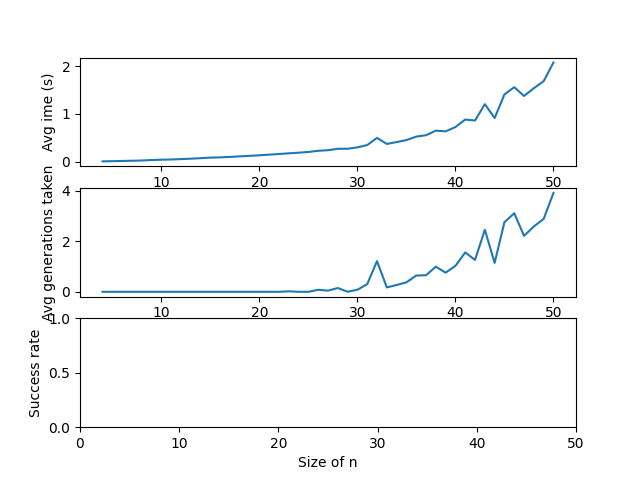
\includegraphics[width=0.8\textwidth]{figure1.png}
    \caption{Main algorithm runtime and generations taken.}
    \label{fig:main}
\end{figure}

\begin{figure}[H]
    \centering
    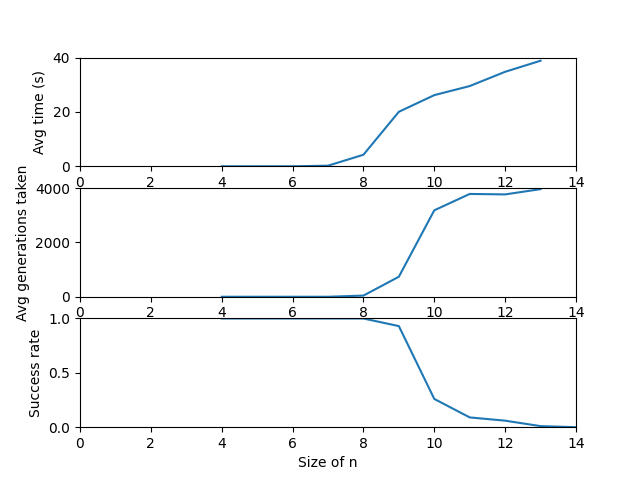
\includegraphics[width=0.8\textwidth]{figure2.png}
    \caption{Simplistic algorithm runtime and generations taken.}
    \label{fig:simplistic}
\end{figure}

\section{Conclusions}
\label{sec:conclusions}

\textcolor{black}{TBA.}

\bibliographystyle{ieeetr}
\bibliography{references}

\end{document}
